
%------------------------------------------------ EXPERIMENTS --------------------------------------------------------
\section{\label{section:experiments} Experiments}

The experiments presented in this section are intended to explore the various properties of both, the Variational
GP-LVM as well as its dynamical version. The most important of these properties include the generative Bayesian
nature of our models, the ability to handle very high dimensional data as well as the automatic way of determining
the complexity and performing model selection.

Therefore, we evaluate the models' performance in a variety of tasks, namely
visualisation, prediction, reconstruction and generation of data or timeseries.
Matlab source code for repeating the following experiments is available
on-line from: \\
\verb|http://staffwww.dcs.shef.ac.uk/people/N.Lawrence/vargplvm/|.

\subsection{Covariance functions used \label{covarianceFunctions}}
Before proceeding to the actual evaluation of our method, we first review and give the forms
of the covariance functions that will be used for our experiments.
The mapping between the input and output spaces $X$ and $Y$ is nonlinear and, thus, we use
the covariance function of equation \eqref{} which also allows simultaneous model selection
within our framework.
In experiments where we use our method to also model dynamics,
apart from the infinitely differentiable squared exponential
covariance function defined in equation \eqref{rbf}, we will also consider for
the dynamical component the Mat\'ern $3/2$ covariance function which is only once
differentiable, and a periodic one
\citep{rasmussen-williams, MacKay98} which can be used when data
exhibit strong periodicity. These covariance functions take the form:
\begin{eqnarray}
%k_{x(\text{rbf})} \left( \mathit{t_i, t_j} \right) 
%& = & \sigma_{\text{rbf}}^2 e^{- \frac{\left( t_i - t_j \right)^2}{\left(
%      2l_t^2 \right)}}, 
k_{x(\text{mat})} \left( t_i, t_j \right)& = &  
\sigma_{\text{mat}}^2 \left( 1 + \frac{\sqrt{3} |t_i - t_j|}{l} \right)
		\exp \left( \frac{ - \sqrt{3} |t_i - t_j|}{l} \right), \nonumber \\
%\label{matern} 
k_{x(\text{per})} \left( \mathit{t_i, t_j} \right) 
& = & 
	\sigma_{\text{per}}^2 \exp \left( -\frac{1}{2} \frac{\sin^2 \left( \frac{2
                \pi}{T} \left( t_i - t_j \right) \right) }{l} \right),
 \label{eq:temporalkernels}
\end{eqnarray}
%
where $l$ denotes the characteristic lengthscale and $T$ denotes the period of the periodic covariance function.
%
\par Introducing a separate GP model for the dynamics is a very convenient way of incorporating any prior information
we may have about the nature of the data in a nonparametric and flexible manner. 
In particular, more sophisticated covariance functions can be constructed
by combining or modifying existing ones. For example, in our experiments we consider a compound covariance function,
$k_{x(\text{per})} + k_{x(\text{rbf})}$
which is suitable for dynamical systems that are known to be only approximately periodic. 
The first term
captures the periodicity of the dynamics whereas the second one corrects for the divergence
from the periodic pattern by enforcing the datapoints to form smooth trajectories in time.
By fixing the two variances, $\sigma_{\text{per}}^2$ and $\sigma_{\text{rbf}}^2$ to particular ratios, we are able
to control the relative effect of each kernel. Example sample paths drawn from this compound covariance function are
shown in figure \ref{fig:rbfPeriodic}.

\begin{figure}[ht]
\begin{center}
\subfigure[]{
	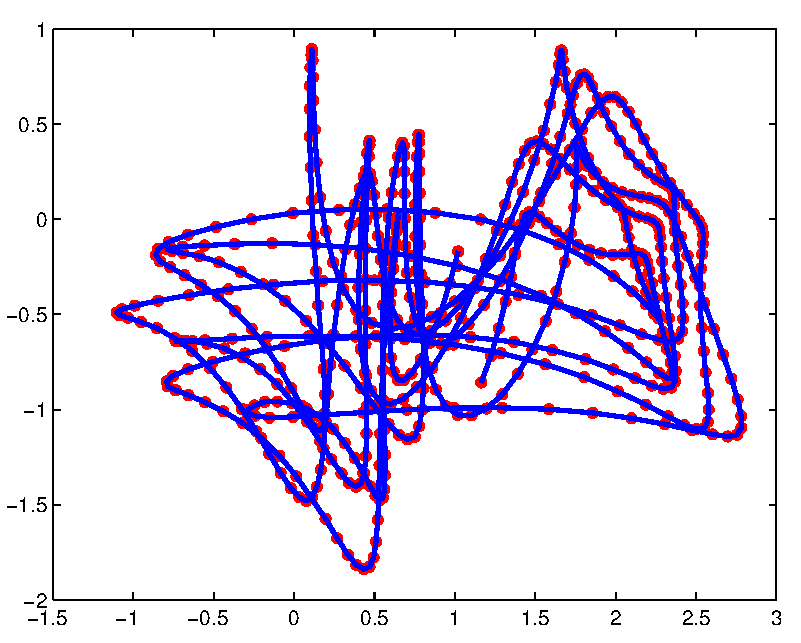
\includegraphics[width=0.31\textwidth]{../diagrams/periodicSamples2}
	\label{fig:rbfPeriodic1}
}
\subfigure[]{
	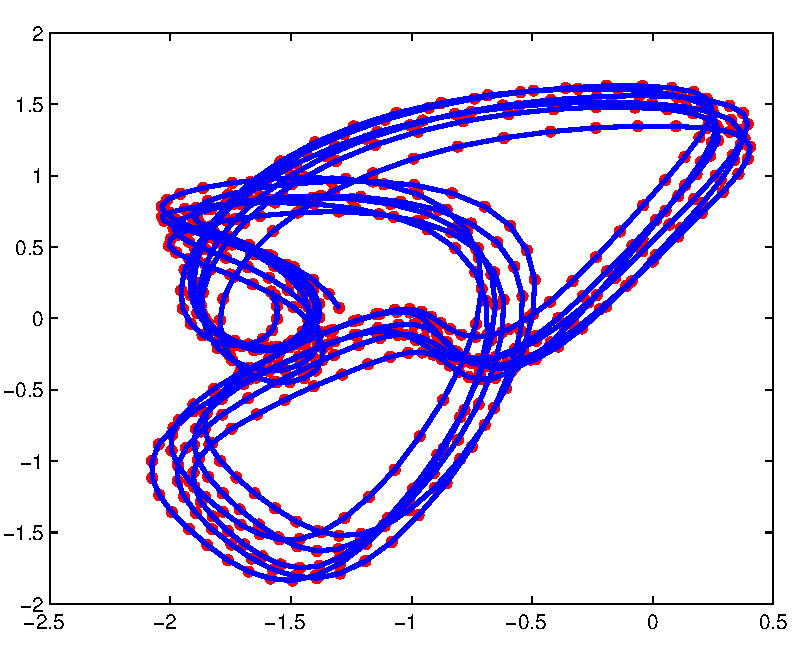
\includegraphics[width=0.31\textwidth]{../diagrams/periodicSamples}
	\label{fig:rbfPeriodic2}
}
\subfigure[]{
	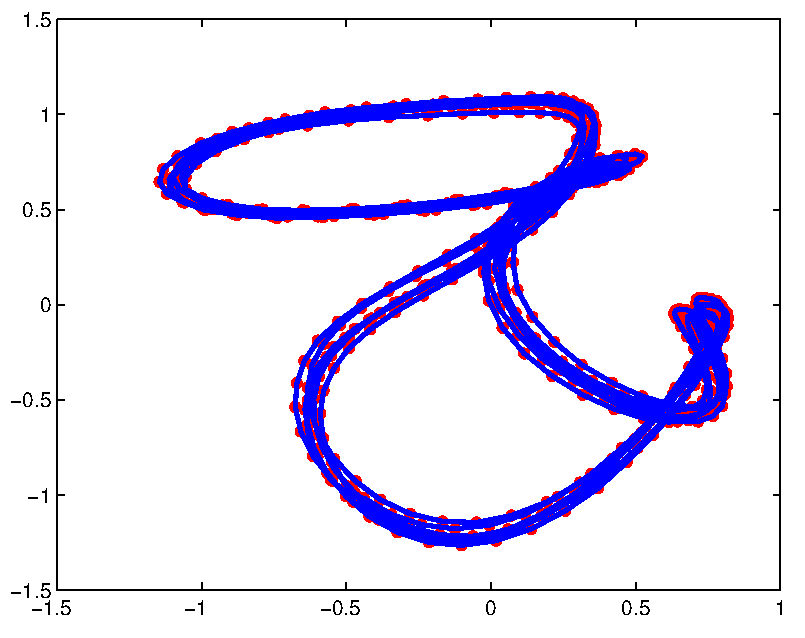
\includegraphics[width=0.31\textwidth]{../diagrams/periodicSamples3}
	\label{fig:rbfPeriodic3}
}
\end{center}
\caption{
  \small{
    Typical sample paths drawn from the $k_{x(\text{per})} + k_{x(\text{rbf})}$ covariance function.
    The variances are fixed for the two terms,
    controlling their relative effect. In figures \subref{fig:rbfPeriodic1}, \subref{fig:rbfPeriodic2} and \subref{fig:rbfPeriodic3},
    the ratio $\sigma_{\text{rbf}}^2 / \sigma_{\text{per}}^2$ of the two variances was large, intermediate and small respectively,
    causing the periodic pattern to be shifted proportionally each period.
  }
}
\label{fig:rbfPeriodic}
\end{figure}

% \par Although the GP-LVM is built on a Gaussian noise model, it is a common tactic to additionally include a white
\par For our experiments we additionally include a noise covariance function 
\begin{equation}
\label{whiteNoise}
k_{white}(\bfx_i, \bfx_j) = \theta_{white} \delta_{ij},
\end{equation}
where $\delta$ is the Kronecker delta function. In that way, we can define a compound 
kernel $k_x + k_{white}$ (and $k_f + k_{white}$ for the GP prior on $f$), so that
the noise level $\theta_{white}$ can be jointly optimised along with the rest of the kernel hyperparameters. Similarly,
one can also include a bias term $\theta_{bias} \mathbf{1}$. %, mostly useful for performing numerically stable computations.

\subsection{Visualisation tasks}

Given a dataset with known structure, we can apply our algorithm and evaluate its performance in a simple and intuitive
way, by checking if the form of the discovered low dimensional manifold agrees with our prior knowledge.
%In this section we present two experiments of this kind. 
\par
%Firstly, we 
We
illustrate the method in the multi-phase oil
flow data \cite{Bishop:oil93} that consists of $1000$, $12$ 
dimensional observations belonging to three known classes
corresponding to different phases of oil flow.   
Figure \ref{fig:oil} shows the results for these  data obtained
by applying the Bayesian GP-LVM with $10$ latent dimensions using the ARD SE
kernel. The means of the variational distribution were initialized
based on PCA, while the variances in the variational distribution are 
initialized to neutral values around $0.5$. As shown in Figure
\ref{fig:oilScales}, the algorithm switches
off $8$ out of $10$ latent dimensions by making their 
inverse lengthscales exactly or close to zero. Therefore, the
two-dimensional nature of this dataset is automatically revealed. Figure \ref{fig:oilBGPLVM} shows the
visualization obtained by keeping only the 
dominant latent directions 
which are the dimensions $2$ and $3$. This is a remarkably high quality two
dimensional visualization of this data. For comparison, Figure
\ref{fig:oilGPLVM} shows the visualization provided by the standard sparse
GP-LVM that runs by a priori assuming only $2$ latent dimensions. 
Both models use $50$ inducing variables, while the latent variables
$X$ optimized in the standard GP-LVM are initialized based on PCA. 
Note that if we were to run the standard GP-LVM with $10$ latent 
dimensions, the model would overfit the data, it would not reduce the 
dimensionality in the manner achieved by the Bayesian GP-LVM. 
The quality of the class separation in the two-dimensional space
can also be quantified in terms of the nearest neighbour error for the different
classes (phases of oil flow): the number of nearest neighbour errors made when applying
the standard GP-LVM was $26$ out of $1000$ points, whereas the Bayesian GP-LVM made only one error.

%In these two dimensions, the nearest neighbour error for the different classes 
%(phases of oil flow) in the case of Bayesian GP-LVM is $1$ error from
%$1000$ data points. The number of the nearest neighbour errors made
%when applying the standard GP-LVM was $26$. 

%%% TODO %%%%
%Due to the curse of dimensionality, it is often difficult to recognise the structure of high dimensional data, even if there is some.
%A dimensinoality reduction algorithm can be useful for visualising this kind of data, so that we can gain some intuition about their nature.
%This is achieved by visualising a low dimensional, non-linear projection of the data. 
%Reversely, given a dataset with known structure, we can apply our algorithm and evaluate its performance in a simple and intuive way by checking if the shape of the discovered low dimensional manifold agrees with our prior knowledge. 
%
%In this section we present two experiments of this kind. Most of the existing approaches cannot ... so they set by hand 2 or 3 latent dims...
%advantage of vargplvm to find the number of latent dims...
%%%%



\begin{figure}[ht]
\begin{center}
\subfigure[]{
	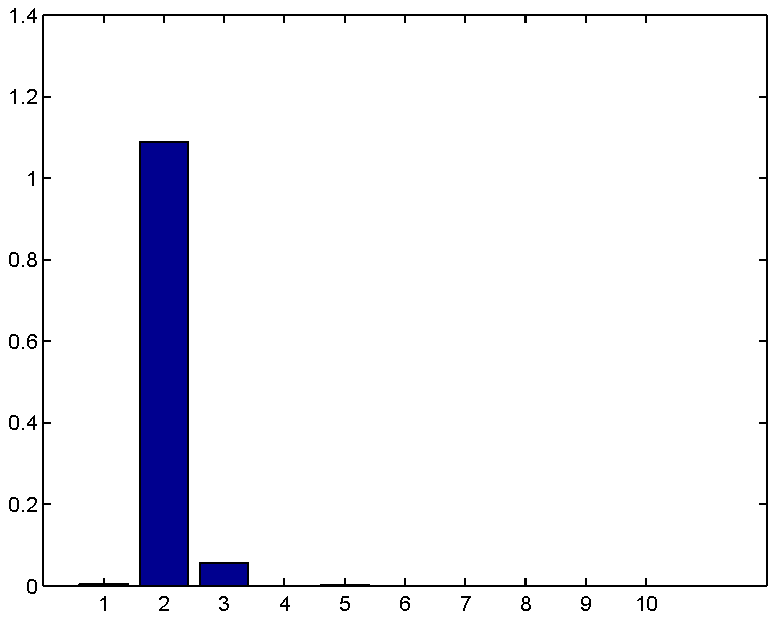
\includegraphics[width=0.31\textwidth]{../diagrams/demOilVargplvm4Scales.pdf}%demOilVargplvm1Scales.pdf
	\label{fig:oilScales}
}
\subfigure[]{
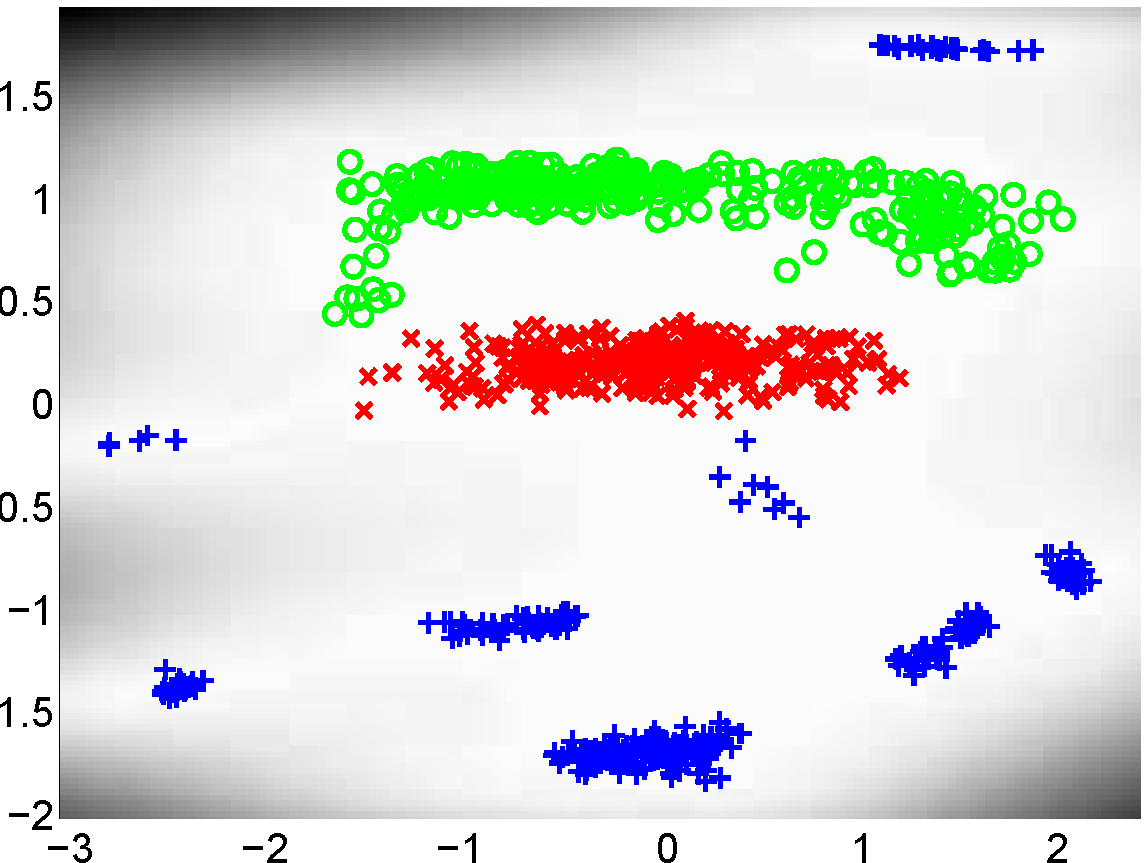
\includegraphics[width=0.31\textwidth]{../diagrams/demOilVargplvm4.pdf} %demOilVargplvm1.pdf
	\label{fig:oilBGPLVM}
}
\subfigure[]{
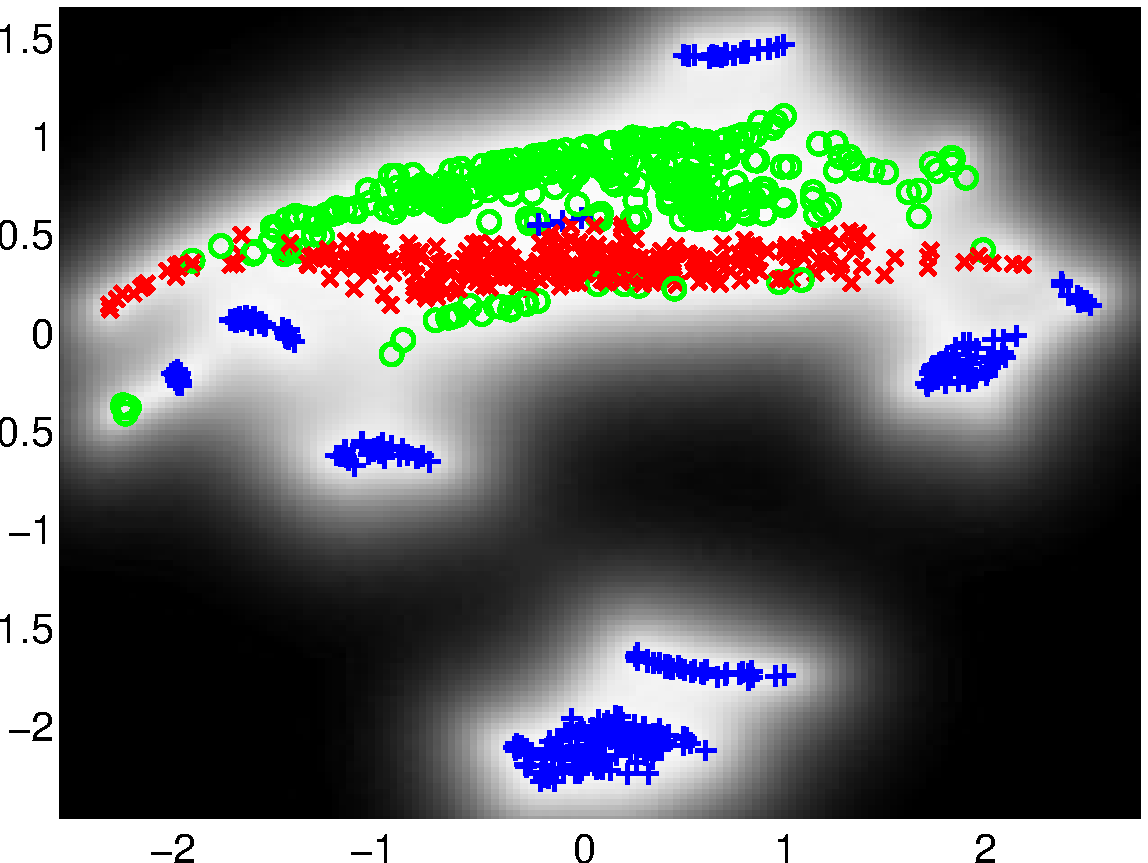
\includegraphics[width=0.31\textwidth]{../diagrams/demOilFgplvm7.pdf}
	\label{fig:oilGPLVM}
}
\end{center}
\caption{\small{
 Panel (a) shows the inverse lengthscales found by applying the
  Bayesian GP-LVM with ARD SE kernel on the oil flow data. Panel (b)
  shows the visualization achieved by keeping the most dominant latent
  dimensions (2 and 3) which have the largest inverse lengthscale
  value. Dimension 2 is plotted on the
  $y$-axis and 3 and on the $x$-axis. Plot (c) shows the visualization found
  by standard sparse GP-LVM.
}
}
\label{fig:oil}
\end{figure}

%%%%%%%% TODO
%\par As a second visualisation task, 
%
%\begin{figure}[ht]
%\begin{center}
%\subfigure[]{
%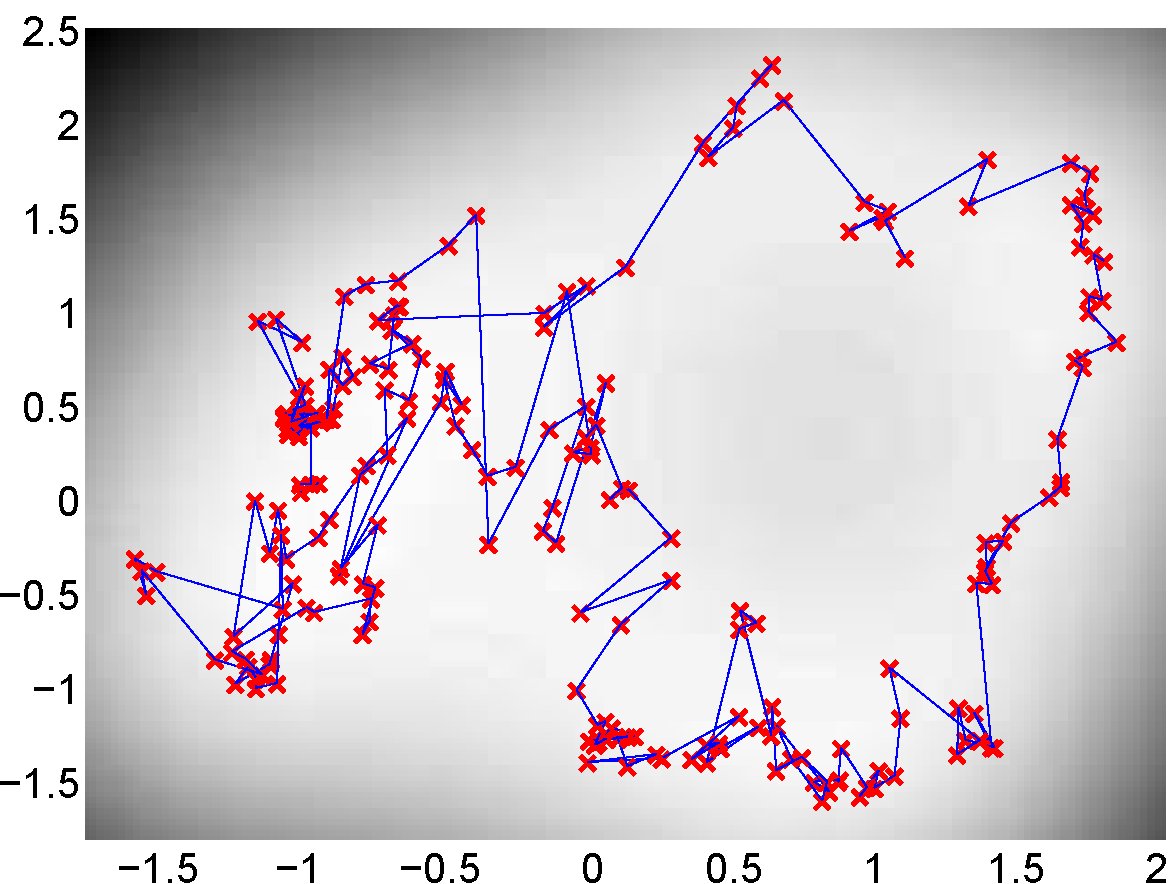
\includegraphics[width=0.45\textwidth]{../diagrams/demRobotWirelessVargplvmStatic.pdf}
%	\label{fig:robotStatic}
%}
%\subfigure[]{
%	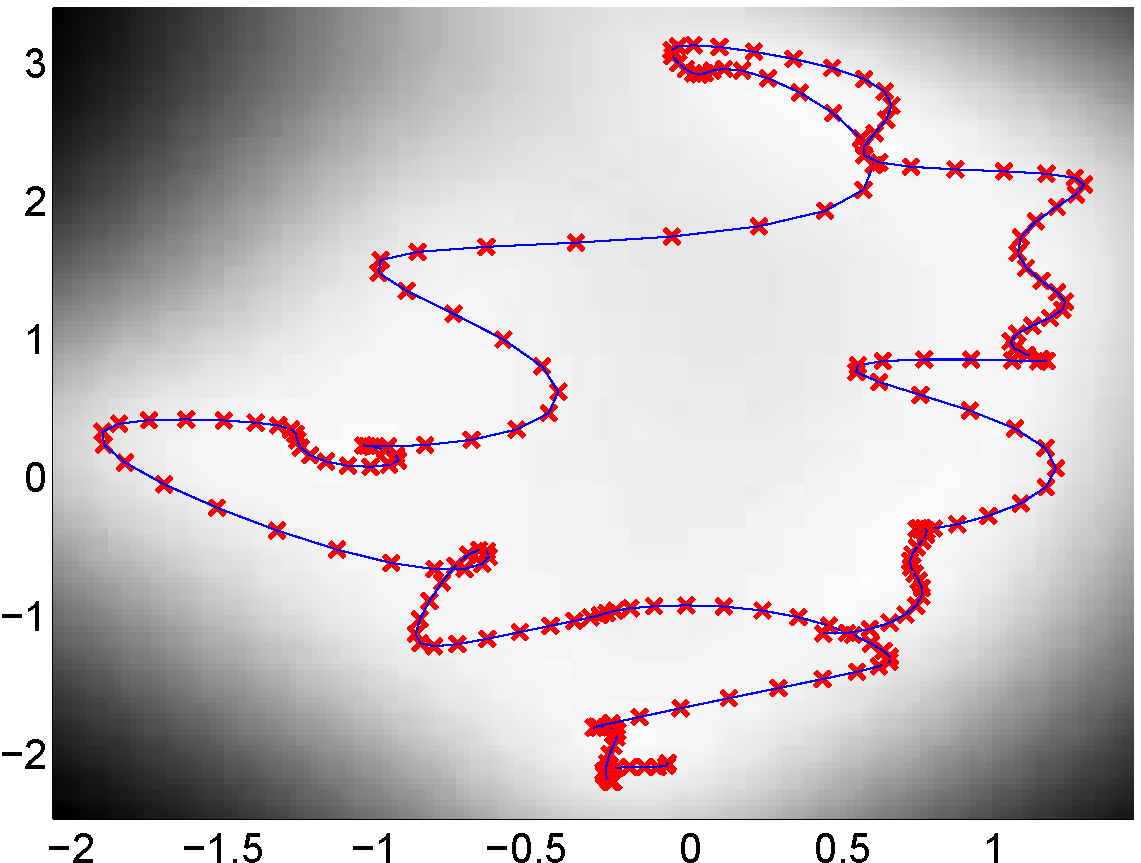
\includegraphics[width=0.45\textwidth]{../diagrams/demRobotWirelessVargplvmDynRbf.pdf}
%	\label{fig:robotDyn}
%}
%\end{center}
%\caption{\small{
%    Loop closure in robotics. \subref{fig:robotStatic}: var. gplvm without dynamics. \subref{fig:robotDyn}: var. gplvm with an RBF kernel to model the dynamics....
%}
%}
%\label{fig:robot}
%\end{figure}

\subsection{Human Motion Capture Data}

We followed \cite{Taylor,gplvmLarger} in considering motion capture
data of walks and runs taken from subject 35 in the CMU motion capture
database. We used the dynamical version of our model and
treated each motion as an independent sequence.  The data
set was constructed and preprocessed as described in
\cite{gplvmLarger}. This results in 2,613 separate 59-dimensional
frames split into 31 training sequences with an average length of 84
frames each. Our model does not require explicit timestamp information, since we
know a priori that there is a constant time delay between poses and the model can construct
equivalent covariance matrices given any vector of equidistant time points.

The model is jointly trained, as explained in section \ref{sequences},
on both walks and runs, i.e. the algorithm learns a common latent
space for these motions. At test time we investigate the ability of
the model to reconstruct test data from a previously unseen sequence
given partial information for the test targets. This is tested once by
providing only the dimensions which correspond to the body of the
subject and once by providing those that correspond to the legs.
%
We compare with results in \cite{gplvmLarger}, which used MAP
approximations for the dynamical models, and against nearest
neighbour. We can also indirectly compare with the binary latent
variable model (BLV) of \cite{Taylor} which used a slightly different
data preprocessing. Furthermore, we additionally tested the non-dynamical
version of our model, in order to explore the structure of the distribution found for the
latent space. In this case, the notion of sequences or sub-motions is not modelled
explicitely, as the non-dynamical approach does not model correlations between
datapoints. However, as will be shown below, the model manages to discover
the dynamical nature of the data and this is reflected in both, the structure of
the latent space and the results obtained on test data.

\par The performance of each method is assessed by using the cumulative
error per joint in the scaled space defined in \cite{Taylor} and by
the root mean square error in the angle space suggested by
\cite{gplvmLarger}. Our models were initialized with nine latent
dimensions. For the dynamical version, we performed two runs, once using the Mat\'ern covariance
function for the dynamical prior and once using the RBF.

%
The appropriate latent space dimensionality for the data was
automatically inferred by our models. 
%If an RBF covariance governed
%the dynamics the model retained four dimensions, whereas the model
%that used the Matern kept only three.
The non-dynamical model
discovered a $5$-dimensional latent space.
The model which employed an Mat\'ern covariance to govern the dynamics retained four dimensions,
whereas the model that used the RBF kept only three. 
%
%The
%models automatically inferred that the
%appropriate latent space dimensionality for the data was three. 
%
The other latent dimensions were completely switched off by the ARD
parameters.



 From table
\ref{motionCaptureTable} we see that the dynamical Variational GP-LVM
considerably outperforms the other approaches.
The best performance for the legs and the body
reconstruction was achieved by the dynamical VGPLVM model that used the Mat\'ern
and the RBF covariance function respectively. This is an intuitive result, since the smoother
body movements are expected to be better modelled using the infinite differentiable
RBF covariance function, whereas the Mat\'ern one can easier fit the rougher leg motion.
However, although it is important to take into account any available information about the nature of
the data, the fact that both models outperform significantly other approaches shows that the Bayesian
training manages successfully to fit the covariance function parameters to the data in any case.
%
%It is also worth mentioning that  \highlight{TODO:likelihood}
%
Furthermore, the non-dynamical variational GP-LVM, not only manages to discover a latent space with a dynamical
structure, as can be seen in figure \ref{fig:cmuLatentSpaceStatic}, but is also proven to be very robust when making predictions. Indeed,
table \ref{motionCaptureTable} shows that the non-dynamical variational GP-LVM typically outperforms Nearest Neigbour
and its performance is comparable to the GP-LVM which explicitely models dynamics but uses MAP approximations.




%The best performance for legs reconstruction was achieved by the model using the Matern covariance whereas the best performance for body reconstruction used the RBF.
\begin{figure}[ht]
\begin{center}
\subfigure[]{
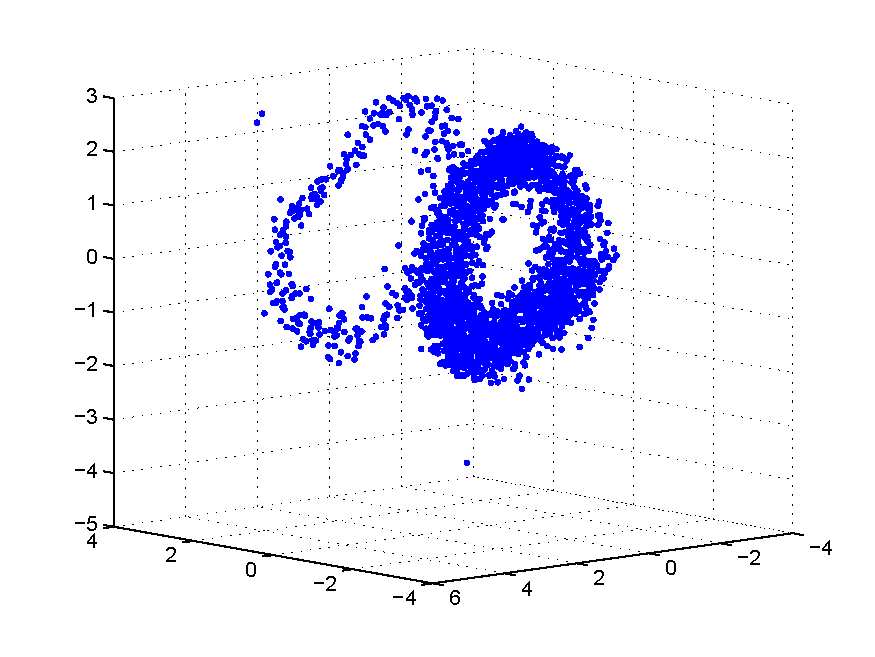
\includegraphics[width=0.31\textwidth]{../diagrams/demCmuStaticLatentSpaceX123}
	\label{fig:cmuLatentSpaceStatic}
}
\subfigure[]{
	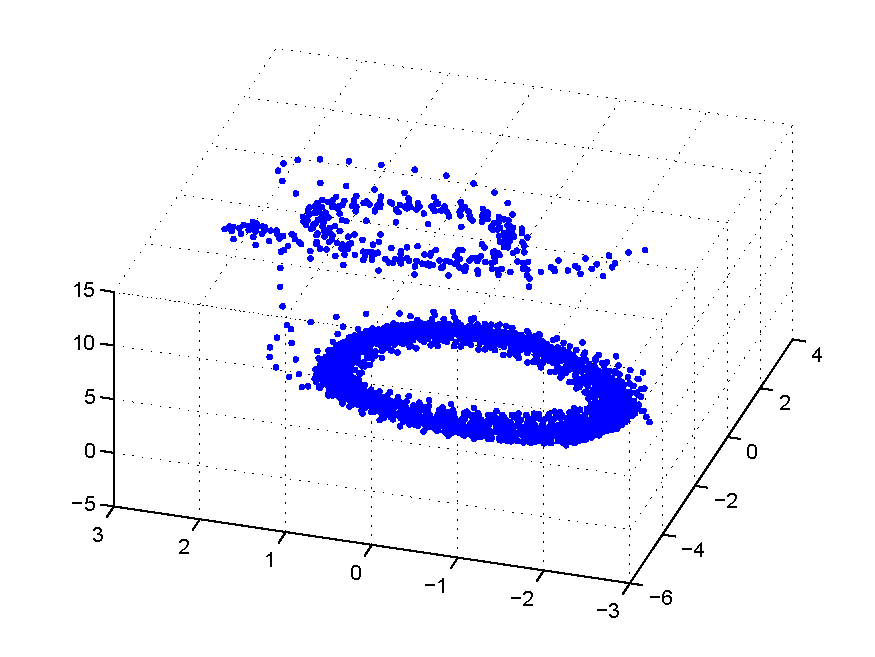
\includegraphics[width=0.31\textwidth]{../diagrams/demCmuMaternLatentSpace}
	\label{fig:cmuLatentSpaceMatern}
}
\subfigure[]{
	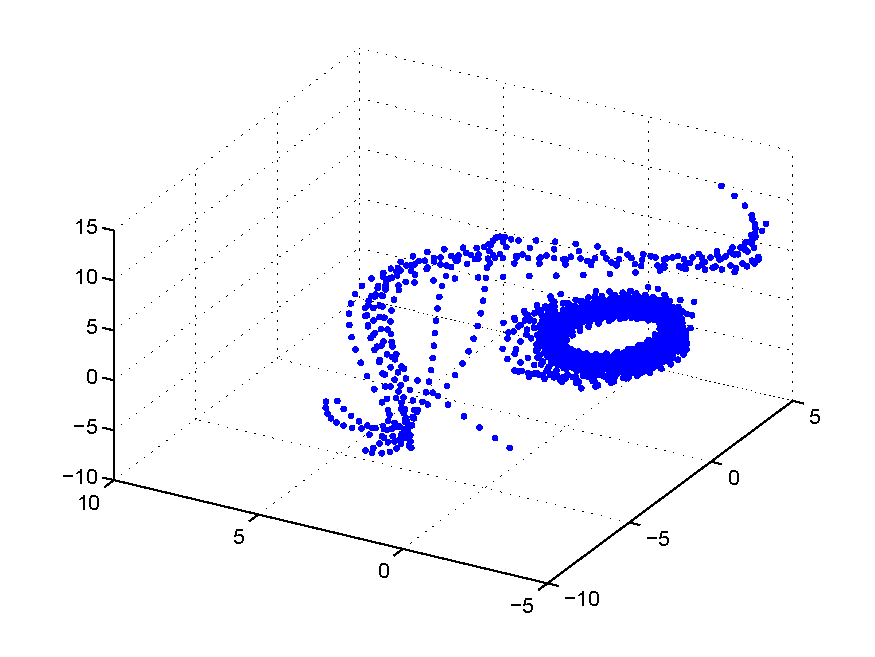
\includegraphics[width=0.31\textwidth]{../diagrams/demCmuRbfLatentSpace}
	\label{fig:cmuLatentSpaceRbf}
}
\end{center}
\caption{\small{
The latent space discovered by our models, projected into its three principle dimensions. The latent space found by the
non-dynamical Bayesian GP-LVM is shown in \subref{fig:cmuLatentSpaceStatic}, by the dynamical model which uses the
Mat\'ern in \subref{fig:cmuLatentSpaceMatern} and by the dynamical model which uses the RBF in \subref{fig:cmuLatentSpaceRbf}.
}
}
\label{fig:cmuLatentSpaces}
\end{figure}


\begin{table}[h]
\caption{
\small{
Errors obtained for the motion capture dataset considering nearest neighbour in the angle space (NN) and in the scaled space(NN sc.), GPLVM, BLV, Variational GPLVM (VGPLVM) and Dynamical VGPLVM (Dyn. VGPLVM). CL / CB are the leg and body datasets as preprocessed in \cite{Taylor}, L and B the corresponding datasets from \cite{gplvmLarger}. SC corresponds to the error in the scaled space, as in Taylor et al. while RA is the error in the angle space. The best error per column is in bold. }}
\label{motionCaptureTable}
\begin{center}
\begin{tabular}{c||c|c|c|c|c|c}
%\multicolumn{1}{c}{\bf PART}  &\multicolumn{1}{c}{\bf DESCRIPTION}
Data & CL & CB & L & L & B & B \\  \hline
Error Type & SC & SC & SC & RA & SC & RA \\
\hline \hline
BLV 			       & 11.7 & \textbf{8.8} & - & - & - & - \\  \hline
NN sc.   		       & 22.2 & \textbf{20.5} & - & - & - & - \\ \hline
GPLVM (Q = 3)	       & - & - & 11.4 & 3.40 & 16.9 & 2.49 \\ \hline
GPLVM (Q = 4)	       & - & - & 9.7  & 3.38 & 20.7 & 2.72 \\ \hline
GPLVM (Q = 5)	       & - & - & 13.4 & 4.25 & 23.4 & 2.78 \\ \hline
NN sc.  		       & - & - & 13.5 & 4.44 & 20.8 & 2.62 \\ \hline
NN 		 	       & - & - & 14.0 & 4.11 & 30.9 & 3.20 \\ \hline
VGPLVM                         & - & - & 14.22& 5.09 & 18.79& 2.79 \\ \hline
Dyn. VGPLVM (RBF)              & - & - & 7.76 & 3.28 & \textbf{11.95} & \textbf{1.90} \\ \hline
Dyn. VGPLVM (Mat\'ern 3/2)     & - & - & \textbf{6.84} & \textbf{2.94} & 13.93 & 2.24 \\
\end{tabular}
\end{center}
\end{table}


%\subsection{TODO}
%\highlight{TODO: Experiment with Jaakko's kernel}

\subsection{Modeling Raw High Dimensional Video Sequences}

For this set of experiments we considered video sequences. Such
sequences are typically preprocessed before modeling to extract
informative features and reduce the dimensionality of the
problem. Here we work directly with the raw pixel values to
demonstrate the ability of the dynamical VGPLVM to model data with a vast number
of features. This also allows us to directly sample video from the
learned model.
\par Firstly, we used the
model to reconstruct partially observed frames from test video
sequences
\footnote{`Missa' dataset: cipr.rpi.edu. `Ocean': cogfilms.com. `Dog': fitfurlife.com.
  See details in supplementary. The logo appearing in the `dog' images in the experiments that follow,
  has been added with post-processing.}.
For the first video discussed here we gave as partial information approximately 
50\% of the pixels while for the other two we gave approximately 40\% of the pixels on each frame.
The mean squared error per pixel was measured to compare
with the $k-$nearest neighbour (NN) method, for $k \in (1,..,5)$ (we
only present the error achieved for the best choice of $k$ in each
case). The datasets considered are the following: firstly, the `Missa'
dataset, a standard benchmark used in image
processing. This is a 103,680-dimensional video, showing a woman talking
for 150 frames. The data is challenging as there are translations in
the pixel space. We also considered an HD video of dimensionality $9
\times 10^5$ that shows an artificially created scene of ocean waves
as well as a $230,400-$dimensional video showing
a dog running for $60$ frames. The later is approximately periodic in
nature, containing several paces from the dog. For the first two
videos we used the Mat\'ern and RBF covariance functions respectively to model the
dynamics and interpolated to reconstruct blocks of frames chosen from
the whole sequence. For the `dog' dataset we constructed a compound
kernel $k_x = k_{x(\text{rbf})} + k_{x(\text{per})}$ presented in section \ref{temporalPrior}, where the
RBF term is employed to capture any divergence from the approximately
periodic pattern. We then used our model to reconstruct the last 7
frames extrapolating beyond the original video. As can be seen in
table \ref{videoResultsTable}, our method outperformed NN in all
cases. The results are also demonstrated visually in figures
\ref{fig:video1} and \ref{fig:dogRec} and the reconstructed videos are available in the supplementary material.


\begin{table}[h]
\caption{
\small{
  The mean squared error per pixel for Dyn. VGPLVM and NN for the three datasets (measured only in the missing inputs).
  The number of latent dimensions selected by our model is in parenthesis. 
} }
\label{videoResultsTable}
\begin{center}
\begin{tabular}{c||l|l|l}
%\multicolumn{1}{c}{\bf PART}  &\multicolumn{1}{c}{\bf DESCRIPTION}
             & Missa & Ocean & Dog \\
\hline \hline
Dyn. VGPLVM  & 2.52 ($Q = 12$) & 9.36 ($Q = 9$)  & 4.01 ($Q = 6$) \\  \hline
NN           & 2.63 & 9.53 & 4.15 \\
\end{tabular}
\end{center}
\end{table}

\begin{figure}[ht]
\begin{center}
\subfigure[]{
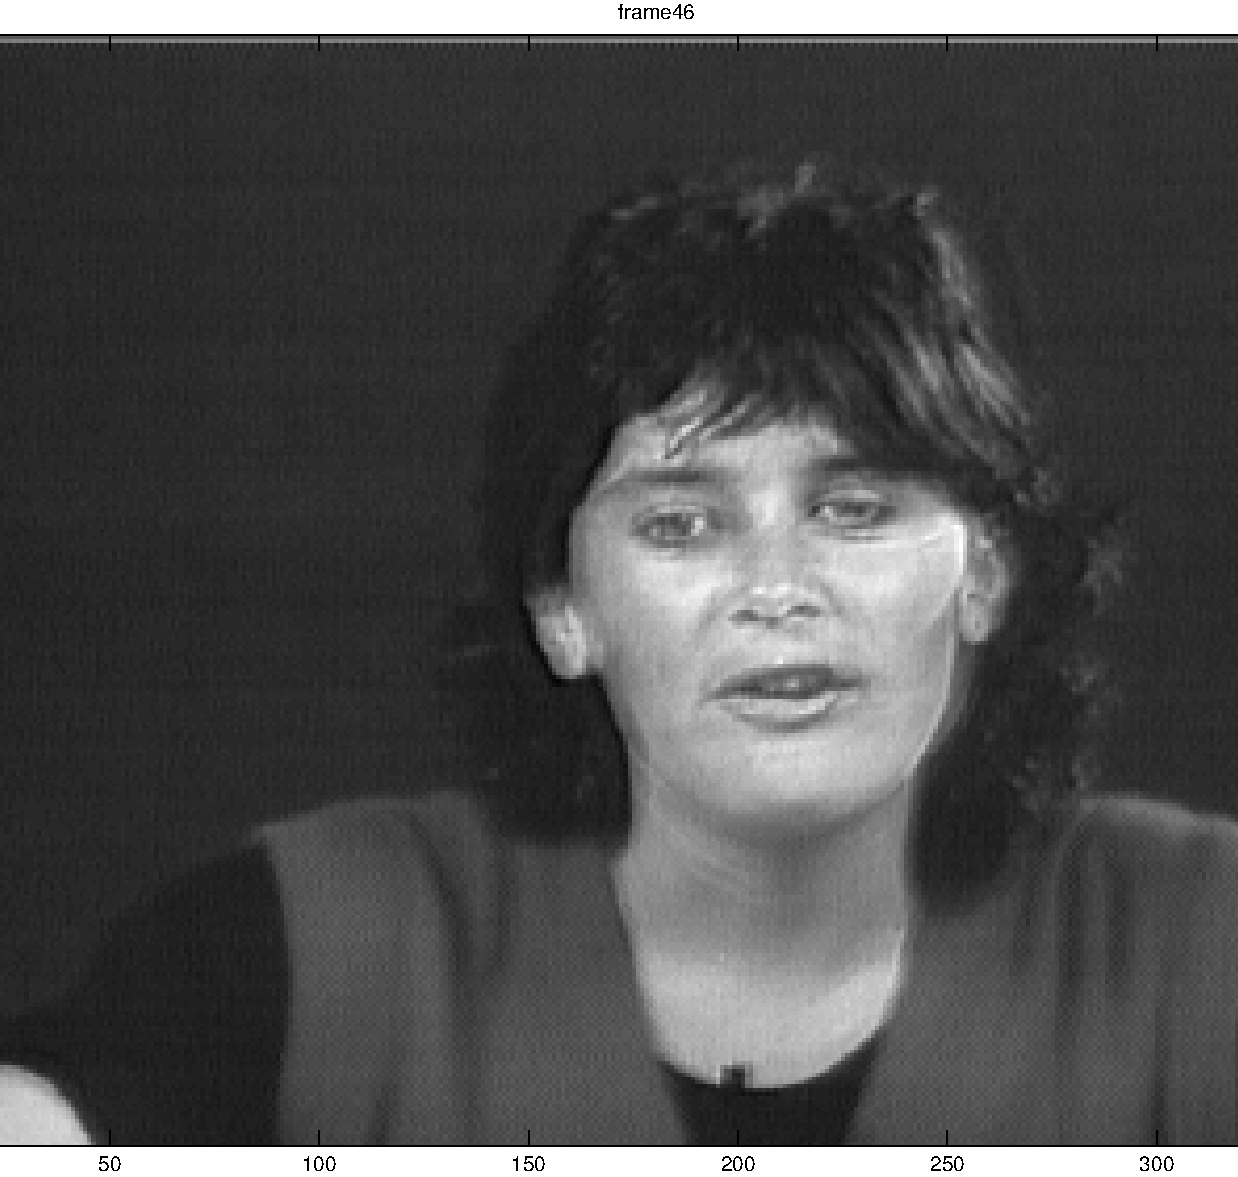
\includegraphics[width=0.24\textwidth]{../diagrams/missaGpdsframe46.pdf}
	\label{fig:missa1}
}
\subfigure[]{
	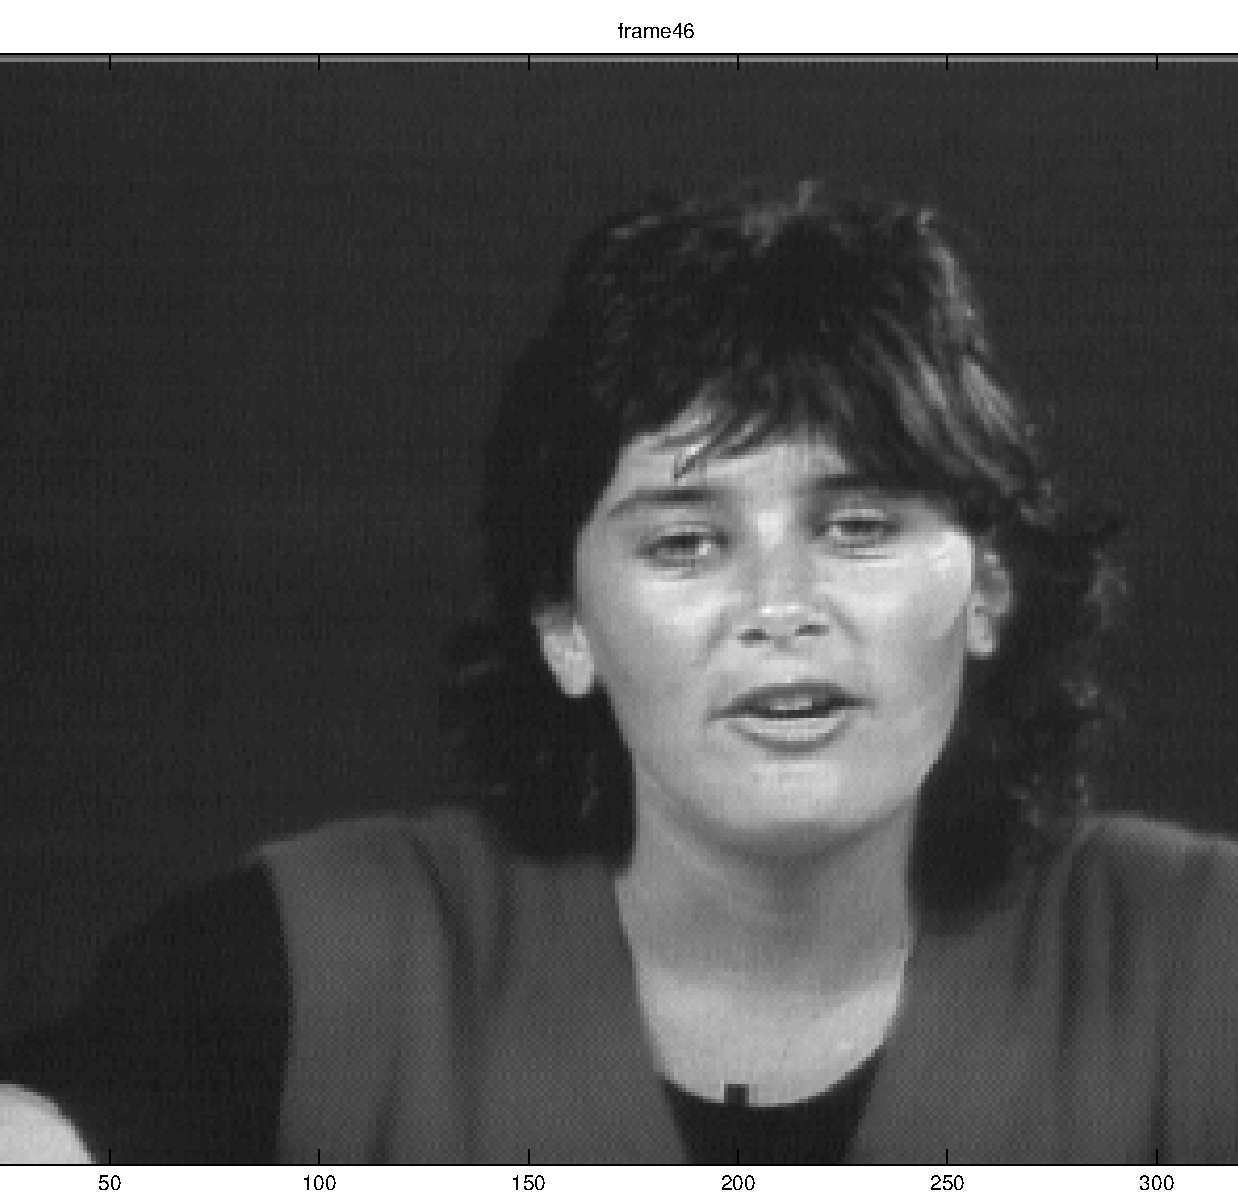
\includegraphics[width=0.24\textwidth]{../diagrams/missaYtsOrigframe46.pdf}
	\label{fig:missa2}
}
\subfigure[]{
	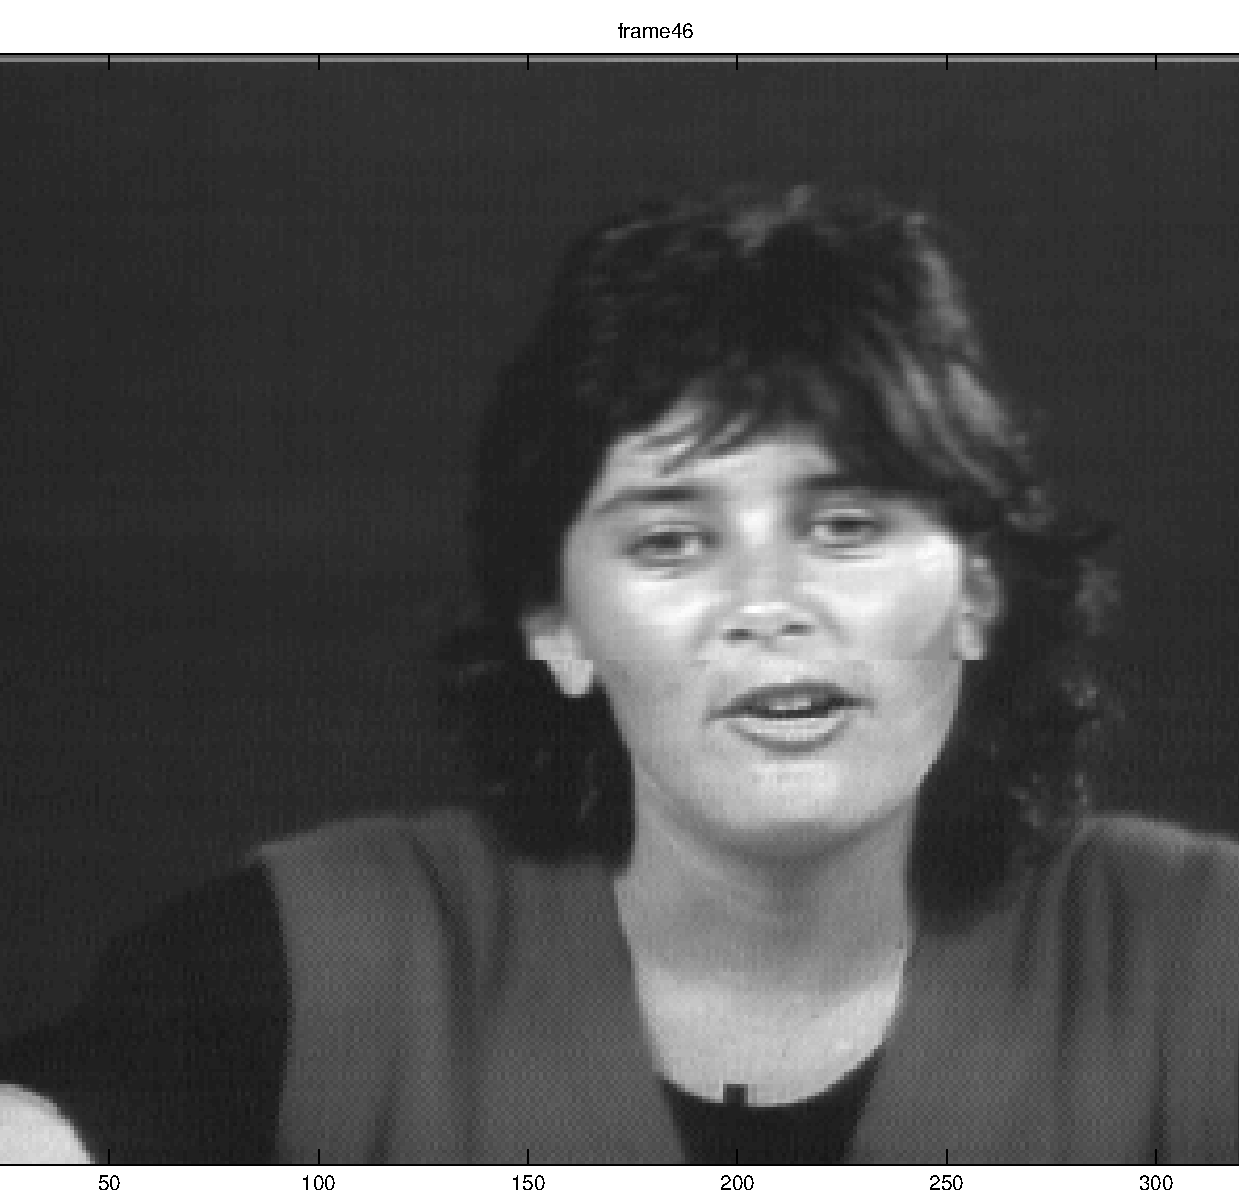
\includegraphics[width=0.24\textwidth]{../diagrams/missaNNframe46}
	\label{fig:missa3}
}
\subfigure[]{
	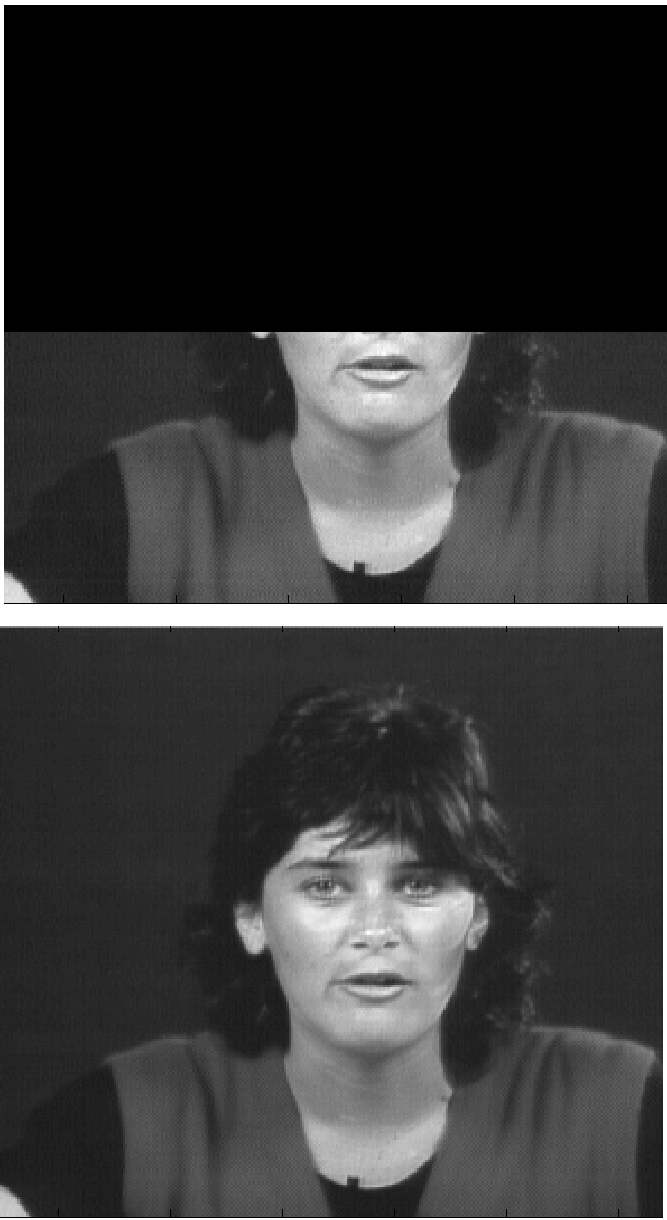
\includegraphics[width=0.12\textwidth]{../diagrams/missaGpdsPredFrame17}
	\label{fig:missa4}
}
\subfigure[]{
	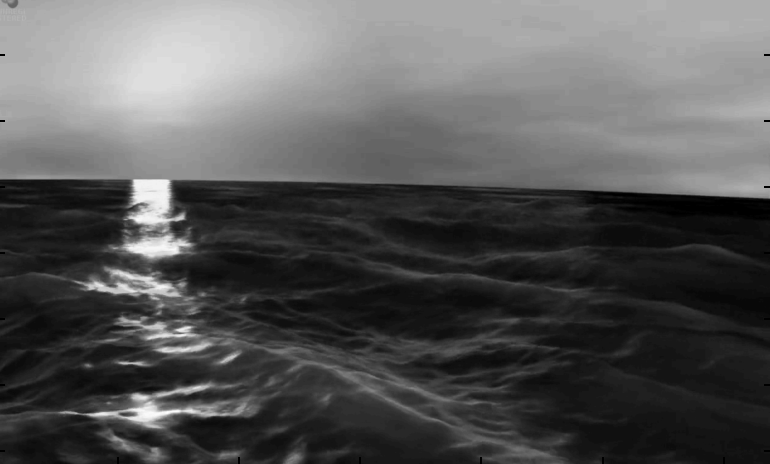
\includegraphics[width=0.39\textwidth]{../diagrams/ocean25_VGPDS}
	\label{fig:ocean1}
}
%\subfigure[]{
%	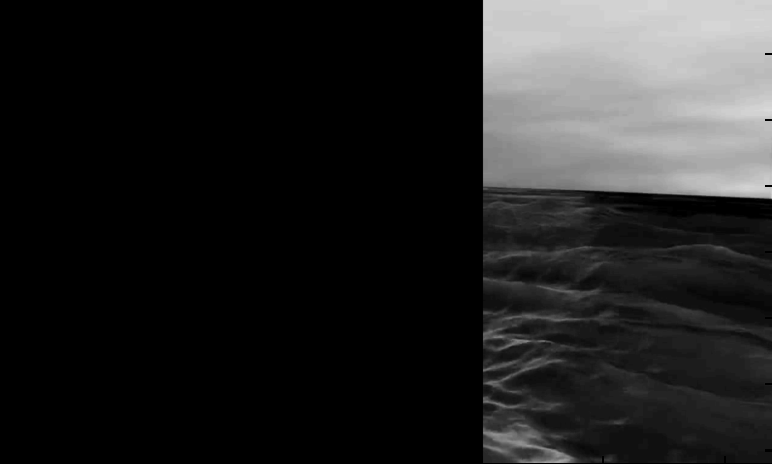
\includegraphics[width=0.28\textwidth]{../diagrams/ocean25_Yts}
%	\label{fig:ocean2}
%}
\subfigure[]{
	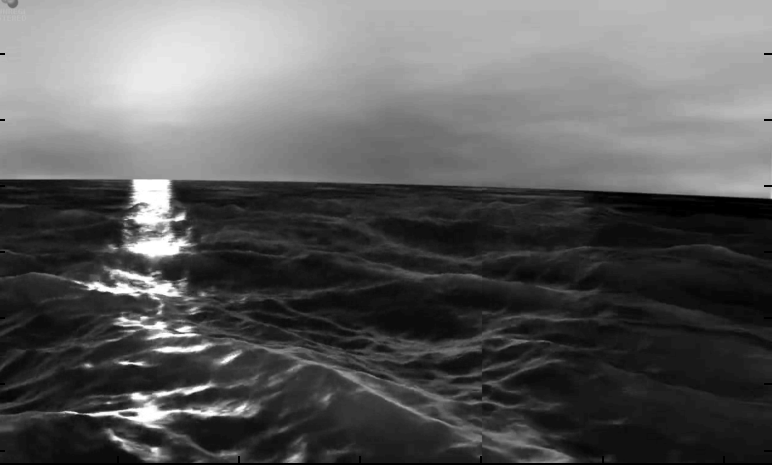
\includegraphics[width=0.39\textwidth]{../diagrams/ocean25_NN}
	\label{fig:ocean3}
}
\subfigure[]{
	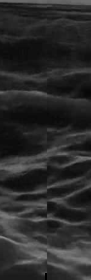
\includegraphics[width=0.08\textwidth]{../diagrams/ocean25_NN_closeup}
	\label{fig:ocean4}
}
      

\end{center}
\caption{\small{
    \subref{fig:missa1} and \subref{fig:missa3} demonstrate the reconstruction achieved by Dyn. VGPLVM and NN respectively for one of the most challenging frames \subref{fig:missa2} of the `missa' video, i.e.\ when translation occurs. \subref{fig:missa4} shows another example of the reconstruction achieved by Dyn. VGPLVM given the partially observed image. \subref{fig:ocean1} (Dyn. VGPLVM) and \subref{fig:ocean3} (NN) depict the reconstruction achieved for a frame of the `ocean' dataset. %, given the partial information shown in figure \subref{fig:ocean2}.
Notice that in both of the aforementioned datasets, our method recovers a smooth image, in contrast to the simple NN (a close up of this problem with NN for the `ocean' video is shown in figure \subref{fig:ocean4}). In contrast to the NN method, which works in the whole high dimensional pixel space, VGPLVM reconstructed the images using a $12$ and a $9$-dimensional compression for the `missa' and the `ocean' video respectively.
}
}
\label{fig:video1}
\end{figure}
As can be seen in figure \ref{fig:video1}, the Dynamical Variational GP-LVM predicts pixels which
are smoothly connected with the observed part of the image, whereas the NN method cannot fit the predicted pixels in the overall context.
This problem with NN is shown in figure \ref{fig:video1}\subref{fig:ocean4}, but it can be seen more evidently in the corresponding video files.

\begin{figure}[ht]
\begin{center}
%\subfigure[]{
%	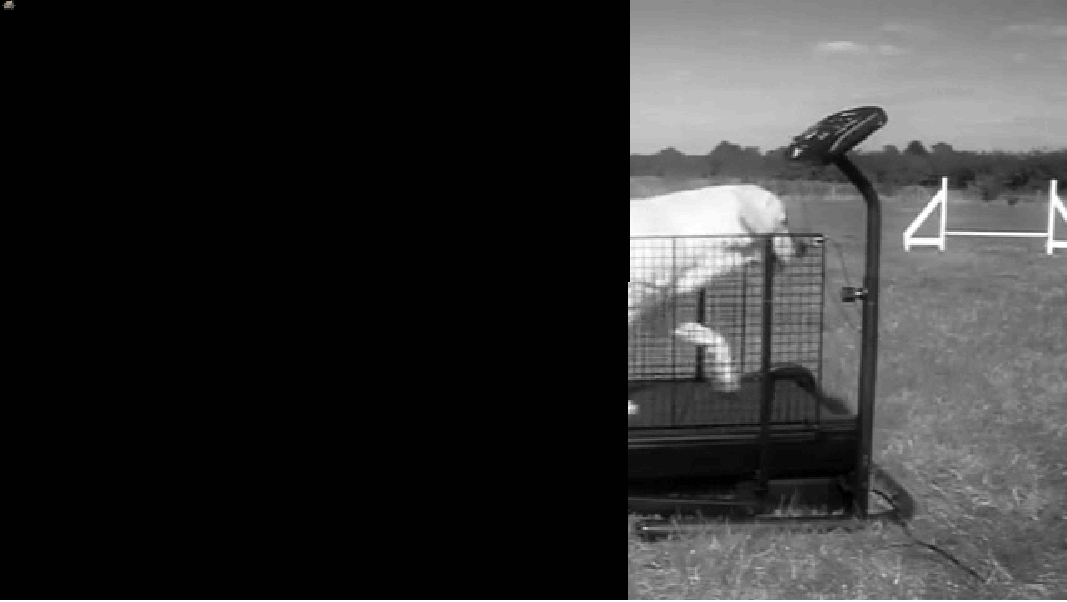
\includegraphics[width=0.23\textwidth]{../diagrams/supplDogPredYts5}
%	\label{fig:suppDog1}
%}
%\subfigure[]{
%	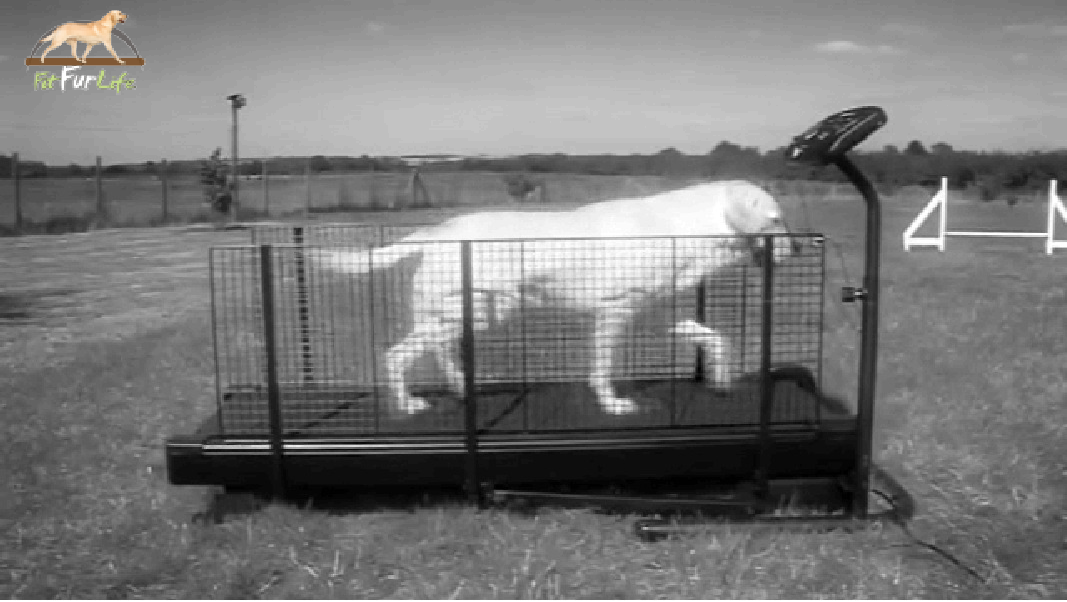
\includegraphics[width=0.23\textwidth]{../diagrams/supplDogPredGpds5}
%	\label{fig:suppDog2}
%}
\subfigure[]{
	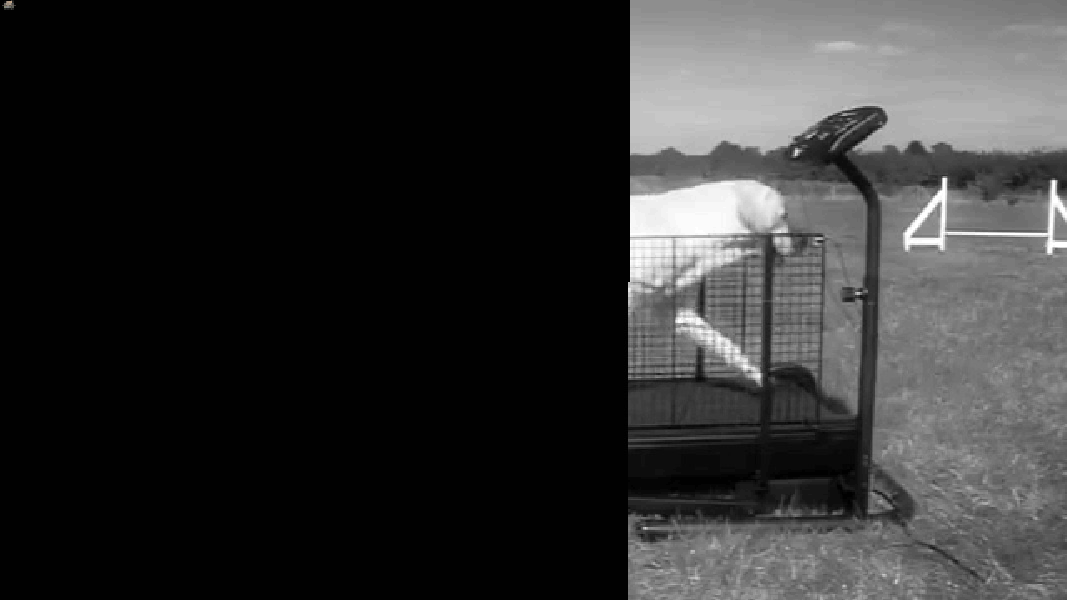
\includegraphics[width=0.23\textwidth]{../diagrams/dogPredYts6}
	\label{fig:dog3}
}
\subfigure[]{
	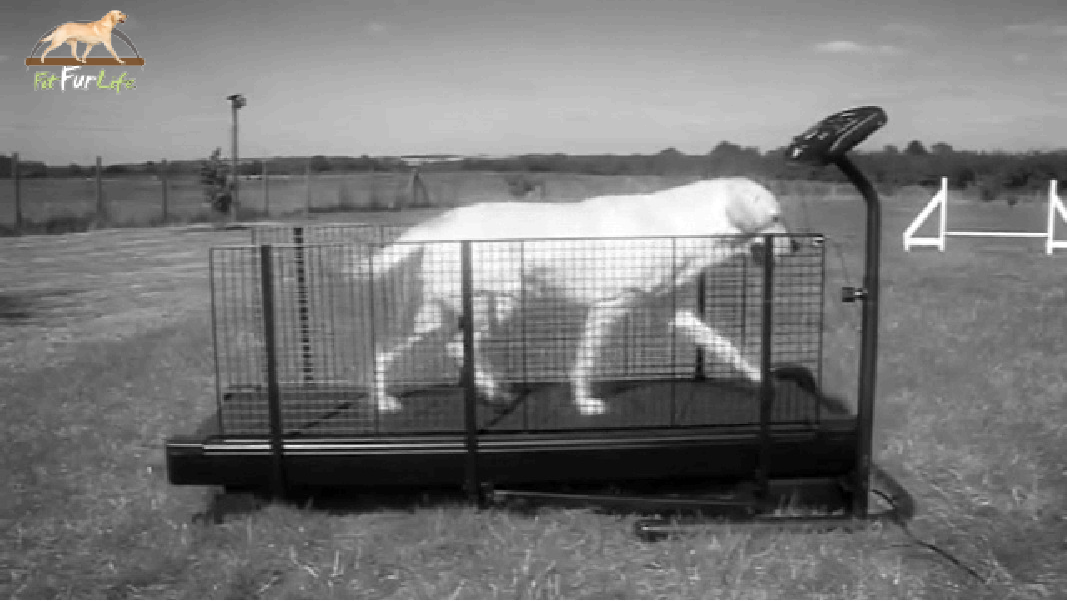
\includegraphics[width=0.23\textwidth]{../diagrams/dogPredGpds6}
	\label{fig:dog4}
}
\subfigure[]{
	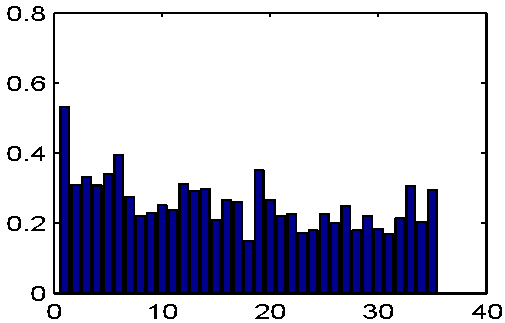
\includegraphics[width=0.23\textwidth]{../diagrams/dog_scalesInit}
	\label{fig:scalesDogInit}
}
\subfigure[]{
	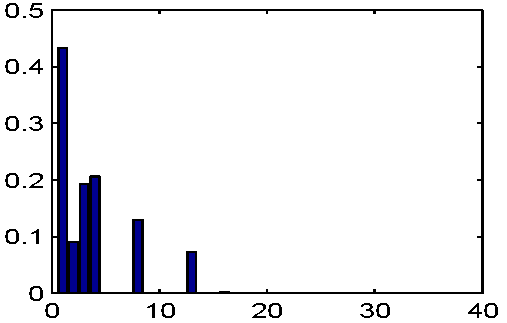
\includegraphics[width=0.23\textwidth]{../diagrams/dog_scalesOpt}
	\label{fig:scalesDogOpt}
}      
\end{center}
\caption{\small{
 An example for the reconstruction achieved for the `dog' dataset. $40\%$ of the test image's pixels (figures \subref{fig:dog3}  were presented  to the model, which was able to successfully reconstruct them, as can be seen in \subref{fig:dog4}.     
Here, we also demonstrate the ability of the model to automatically select the latent dimensionality by showing the initial lengthscales (fig: \subref{fig:scalesDogInit}) of the ARD covariance function and the values obtained after training (fig: \subref{fig:scalesDogOpt}) on the `dog' data set.
}
}
\label{fig:dogRec}
\end{figure}

%\highlight{TODO:} Show what the Latent space represents (maybe can create video from sampling along each of the retained dimensions).

\par As a second task, we used our generative model to create new
samples and generate a new video sequence. This is most effective for
the `dog' video as the training examples were approximately periodic
in nature. The model was trained on 60 frames (time-stamps $[t_1,
t_{60}]$) and we generated new frames which correspond to the next
40 time points in the future. The only input given for this generation
of future frames was the time-stamp vector, $[t_{61}, t_{100}]$. The
results show a smooth transition from training to test and amongst the
test video frames. The resulting video of the dog continuing to run is
sharp and high quality. This experiment demonstrates the ability of
the model to reconstruct massively high dimensional images without
blurring. Frames from the result are shown in figure
\ref{fig:dog}. The full video is available in the supplementary
material.


\begin{figure}[ht]
\begin{center}
\subfigure[]{
	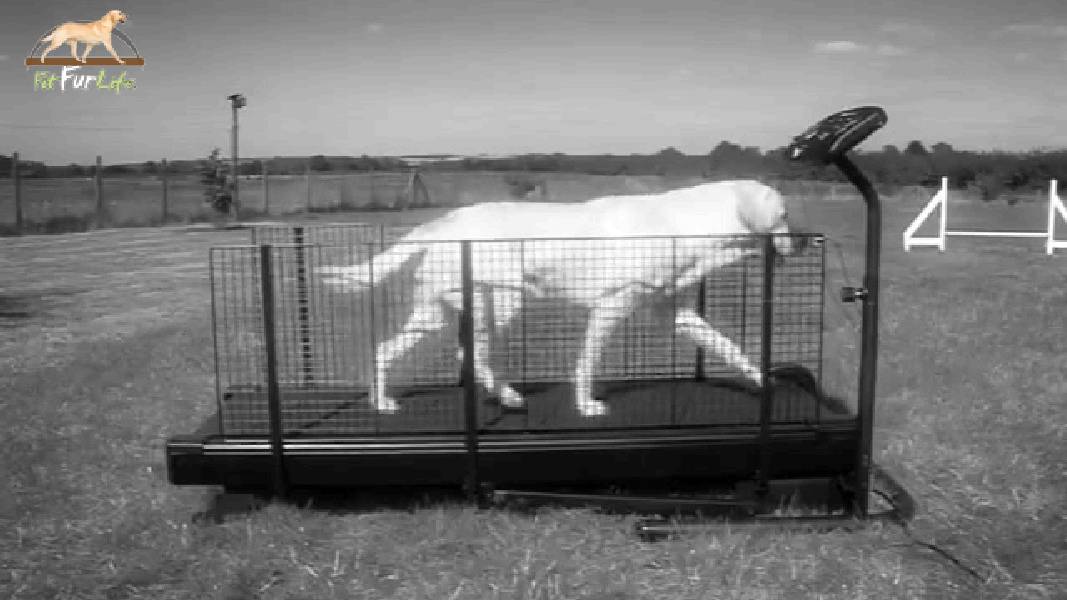
\includegraphics[width=0.23\textwidth]{../diagrams/dogGeneration_lastOfTraining}
	\label{fig:dogTrain}
}
\subfigure[]{
	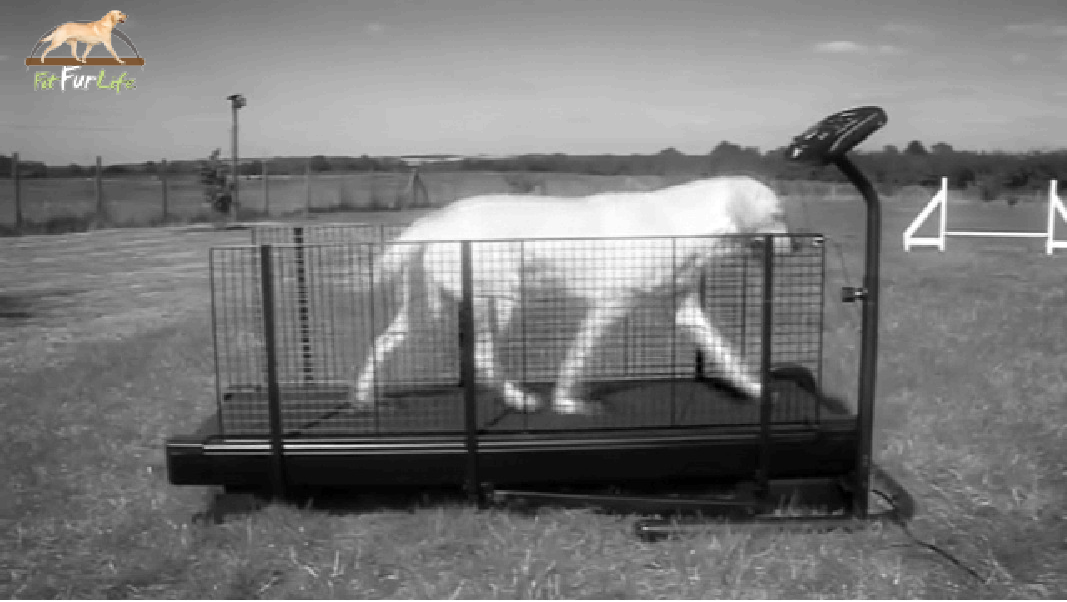
\includegraphics[width=0.23\textwidth]{../diagrams/dogGeneration_firstOfTest}
	\label{fig:dogTest1}
}
\subfigure[]{
	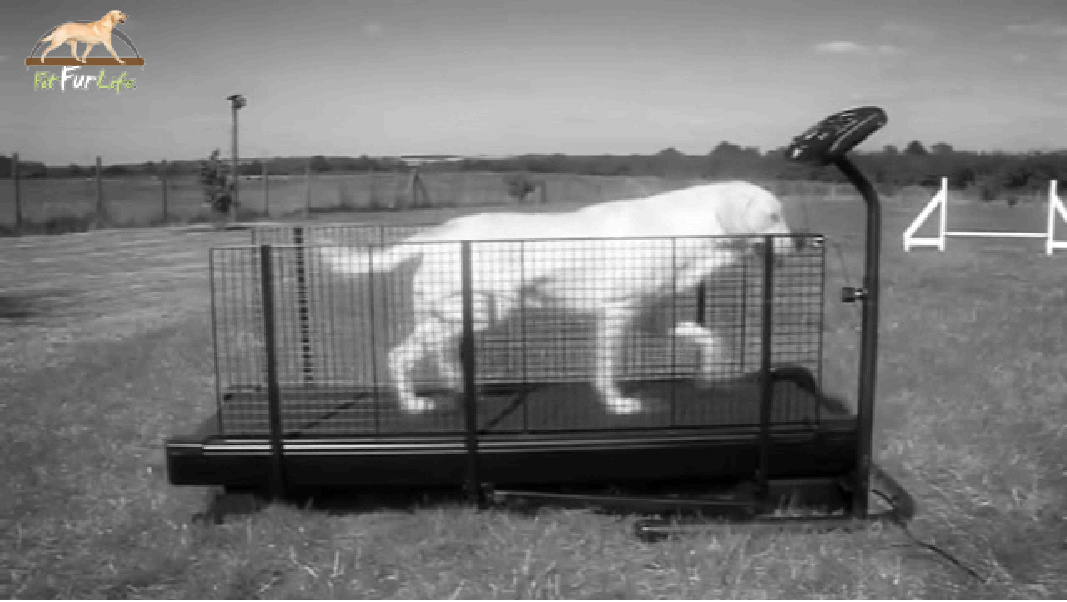
\includegraphics[width=0.23\textwidth]{../diagrams/dogGeneration_frame14}
	\label{fig:dogTest2}
}
\end{center}
\caption{ \small{
The last frame of the training video \subref{fig:dogTrain} is smoothly followed by the first frame \subref{fig:dogTest1} of the generated video. A subsequent generated frame can be seen in \subref{fig:dogTest2}}.}
\label{fig:dog}
\end{figure}


\subsection{Classification}

\highlight{TODO:} This will be pretty much copied from the section ``Digits data'' of the AISTATS paper...

In the final experiment we use the Bayesian GP-LVM to
build a generative classifier for handwritten digit recognition.
We consider the well known USPS digits dataset. This
dataset consists of $16 \times 16$ images for all $10$ digits and it
is divided into $7291$ training examples and $2007$ test examples.
We run $10$ Bayesian GP-LVMs, one for each digit,
on the USPS data base. We used $10$ latent dimensions and
$50$ inducing variables for each model. This allowed us to
build a probabilistic generative model for each digit so that
we can compute Bayesian class conditional densities in the
test data having the form $p(\bfy|Y, digit)$. These class conditional
densities are approximated through the ratio of lower
bounds in eq. \highlight{TODO} as described in section \highlight{TODO}. The whole approach
allows us to classify new digits by determining the
class labels for test data based on the highest class conditional
density value and using a uniform prior over class
labels. The test error made by the Bayesian GP-LVMin the
whole set of $2007$ test points was $95$ incorrectly classified
digits \ie $4.73\%$ error.



\subsection{Bayesian model selection \label{BayesnaModelSelectionExperiments}}

\highlight{TODO} \textit{Maybe this should be merged with the ``classification'' section above}

Being able to (approximately) compute the marginal likelihood $p(Y | \mathcal{M})$ 
is advantageous because it leads to a fully Bayesian training procedure of the model $\mathcal{M}$.
Here, by $\mathcal{M}$ we may refer, for example, to the choice of whether to explicitly model
dynamics or not, or even to the specific kernel selected for the
dynamical priors discussed in section \ref{temporalPrior}.
This means that Bayesian model selection is possible, \ie the value of the optimised marginal likelihood
can be used as an estimator of the quality of the selected model with respect to the
training data $Y$ and, hopefully, to unseen data assumed to have come from the same distribution
$p(Y)$. Unfortunately, however, optimising a lower bound on the marginal likelihood is a non-convex
problem, and the Bayesian model selection can be trusted only under the assumption that the optimisation
algorithm can find good and equivalent local optima for every candidate model $\mathcal{M}$.

Indeed, although we do not claim that the optimised marginal likelihood is a $100\%$ accurate estimator
of the model quality, we present a few simple experiments that confirm that it can, at least, provide an 
idea about what is a good model to use given a dataset $Y$. A more accurate, but also much more
computationally inefficient method would be to perform cross-validation.

Firstly, ...
\highlight{TODO:} \\
(1) \highlight{TODO:} CMU experiment: bounds for static vs dynamical model \\
(2) \highlight{TODO:} Permutation test on the CMU experiment (shuffle timestamps) \\
(3) \highlight{TODO:} Oil data with dynamical model: dynamical kernel's variance goes to 0 and the bound is higher (and performance worse)



\subsection{GP regression with uncertain inputs}
\highlight{TODO}

